\documentclass[ucs, notheorems, handout]{beamer}

\usetheme[numbers,totalnumbers, nologo]{Statmod}
\usefonttheme[onlymath]{serif}
\setbeamertemplate{navigation symbols}{}

\mode<handout> {
	\usepackage{pgfpages}
	%\setbeameroption{show notes}
	%\pgfpagesuselayout{2 on 1}[a4paper, border shrink=5mm]
	\setbeamercolor{note page}{bg=white}
	\setbeamercolor{note title}{bg=gray!10}
	\setbeamercolor{note date}{fg=gray!10}
}

\usepackage[utf8x]{inputenc}
\usepackage[T2A]{fontenc}
\usepackage[russian]{babel}
\usepackage{tikz}
\usepackage{ragged2e}

\newtheorem{theorem}{Теорема}
\newtheorem*{definition}{Определение}
\newtheorem{lemma}{Лемма}
\usepackage{amsmath}
\usepackage{amsthm}
\usepackage{bm}
\usepackage{bbold}

\usepackage{pgfplots}
\pgfplotsset{compat=1.9}

\usepackage{graphicx}
%\usepackage[usenames]{color}
%\usepackage{colortbl}

%\newtheorem{theorem}{Теорерма}
\newtheorem{corollary}[theorem]{Следствие}
%\newtheorem{lemma}[theorem]{Лемма}
\newtheorem{observation}[theorem]{Observation}
\newtheorem{proposition}[theorem]{Предложение}
%\newtheorem{definition}[theorem]{Определение}
\newtheorem{claim}[theorem]{Утверждение}
\newtheorem{fact}[theorem]{Факт}
\newtheorem{assumption}[theorem]{Предположение}
\newtheorem{alg}{Алгоритм}
\newtheorem{zam}{Замечание}

\newtheorem{example}{Пример}[section]

\newenvironment{Proof}{\par\noindent{\bf Доказательство.}}{\hfill$\scriptstyle\blacksquare$}
\newenvironment{ex}{\par\noindent{\bf Пример.}}{}
\newenvironment{pr1}{\par\noindent{\bf Дано:}}{}
\newenvironment{pr2}{\par\noindent{\bf Шаги:}}{}
\newenvironment{pr3}{\par\noindent{\bf Результат:}}{}

\DeclareMathOperator{\tr}{tr}
\DeclareMathOperator{\F}{\mathsf{F}}

\title[Замена непрерывного распределения]{Замена непрерывного распределения на дискретное для применения на практике}
\author[Нагуманова~К. И.]{ Нагуманова Карина Ильнуровна, 19Б.04-мм}

\date{\tiny{Санкт-Петербург\\ 2023г.}}
\institute[Санкт-Петербургский Государственный Университет]{%
	\small
	Санкт-Петербургский государственный университет\\
	Прикладная математика и информатика\\
	Вычислительная стохастика и статистические модели\\
	\vspace{1.25cm}}
\begin{document}
	
	\begin{frame}
		\titlepage
		\note{Научный руководитель  д.ф.-м.н., доцент Голяндина Н.\,Э.,\\
			кафедра статистического моделирования}
	\end{frame}

	\begin{frame}{Введение}
			В практических задачах часто требуется заменить непрерывное распределение на
			дискретное с сохранением математического ожидания и дисперсии. Одним из методов
			нахождения такого распределения для аппроксимации нормального распределения является \textcolor{blue}{\hbox{\textbf{метод Свонсона}}}.
			
			\bigskip
			
			Однако в ряде областей, например, в нефтяной промышленности распределением, описывающим запасы нефти, общепринятым является логнормальное распределение. 
			Соответственно, реальной задачей является аппроксимация логнормального распределения.
	\end{frame}

\begin{frame}{Введение}
	
		Аппроксимируемые случайные величины складывают и умножают.
		
		\bigskip
		
		\textcolor{blue}{\hbox{Пример перемножения:}} используем площадь дренирования пласта, среднюю чистую толщину и коэффициент извлечения углеводородов. При перемножении этих параметров получаем количество резервов нефти.
		
		\bigskip
		
		\textcolor{blue}{\hbox{Пример сложения:}} зная запасы, параметры нефти и породы для всех залежей можно оценить профиль добычи нефти  с каждой залежи и суммарный профиль, оценить экономическую эффективность проекта, которая учитывает выручку, налоги, капитальные затраты, операционные затраты, оптимальные решения по проекту.
		
		\bigskip
		
		\textbf{Задача:} находить аппроксимацию суммы и произведения по аппроксимациям исходных случайных величин.
	
\end{frame}

\begin{frame}{Введение}
	\textbf{Структура работы.}
	\begin{itemize}
		\item В \textbf{разделе 2} рассмотрен общий подход к трехточечной аппроксимации.
		\item В \textbf{разделе 3} аппроксимация нормального распределения, вывод правила 30-40-30.
		\item В \textbf{разделе 4} рассматривается аппроксимация логнормального распределения, два метода, условие аппроксимации и что делать, если это условие не выполняется. А также точность аппроксимации при применении правила 30-40-30 к логнормальному распределению.
		\item В \textbf{разделе 5} алгоритм аппроксимации произведения двух логнормальных распределений.
		\item В \textbf{разделе 6} алгоритм аппроксимации суммы двух логнормальных распределений.
	\end{itemize}
\end{frame}
	
	\begin{frame}{Введение}
		$\xi$ "--- непрерывная случайная величина с математическим ожиданием $m$, дисперсией $s^{2}$ и функцией распределения $F(x)$. Для неё заданы квантили $x_{\pi_{1}}$, $x_{\pi_{2}}$, $x_{\pi_{3}}$. Также есть случайная дискретная величина $\xi_{n}$ с математическим ожиданием $m_{n}$ и дисперсией $s^{2}_{n}$.
		\[\xi_{n}:\quad\begin{pmatrix} 
			x_{\pi_{1}}&x_{\pi_{2}}&x_{\pi_{3}}\\ 
			p_{1} &  p_{2}  & p_{3}
		\end{pmatrix}\]
		Нужно аппроксимировать распределение случайной величины $\xi$ дискретным распределением $\xi_{n}$.
		
		\begin{equation*}
			p_{1} + p_{2} + p_{3} = 1, \label{1}
		\end{equation*}
		\begin{equation*}
			m_{n} = p_{1}x_{\pi_{1}} + p_{2}x_{\pi_{2}} + p_{3}x_{\pi_{3}} = m, \label{2}
		\end{equation*}
		\begin{equation*}
			s_{n}^{2} = p_{1} x_{\pi_{1}}^{2} + p_{2} x_{\pi_{2}}^{2} + p_{3} x_{\pi_{3}}^{2} - m^{2} = s^{2}. \label{3}
		\end{equation*}
		
		
		\note{Постановка задачи в общем виде. Основные обозначения.}
	\end{frame}

\begin{frame}{Условия аппроксимации в общем случае}
	\begin{proposition}\label{pr1}
		Пусть верно 
		\begin{equation*}
			\begin{pmatrix} 
				1&1&1\\ 
				\tilde{x}_{\pi_{1}}~~ &  \tilde{x}_{\pi_{2}}~~  & \tilde{x}_{\pi_{3}} \\ 
				\tilde{x}_{\pi_{1}}^{2}~~&\tilde{x}_{\pi_{2}}^{2}~~  &\tilde{x}_{\pi_{3}}^{2}
			\end{pmatrix}
			\begin{pmatrix}p_{1}\\p_{2}\\ p_{3}\end{pmatrix}= \begin{pmatrix}1\\0\\1 \end{pmatrix},\label{4}
		\end{equation*}
		где $\tilde{x}_{\pi_{i}} = \tilde{\F}^{-1}(\pi_{i})$, $\tilde{\F}(y)$ "--- функция распределения $\displaystyle{\eta = \frac{\xi-m}{s}}$. Тогда $m=m_{n}$ и $s^{2} = s_{n}^{2}$.
	\end{proposition}
\textbf{\textit{Доказательство:}}
\begin{align*}
	\mathsf{P}\left(\frac{\xi-m}{s}\leq \frac{x_{\pi_{i}}-m}{s}\right) &=  \tilde{\F}\left(\frac{x_{\pi_{i}}-m}{s}\right)=\pi_{i},
\end{align*}
\begin{equation*}
	\tilde{x}_{\pi_{i}} = \dfrac{x_{\pi_{i}}-m}{s}=\tilde{\F}^{-1}(\pi_{i}). \label{5}
\end{equation*}
\end{frame}

\begin{frame}{Условия аппроксимации в общем случае}
	Предположим, что $m=m_{n}$ и $s^{2} = s_{n}^{2}$, и получим систему для  вероятностей.
	Для этого подставим $\tilde{x}_{\pi_{i}}$ в формулу мат.ожидания, получаем
	\begin{equation*}
		m(p_{1} + p_{2} + p_{3})+s(p_{1}\tilde{x}_{\pi_1}+p_{2}\tilde{x}_{\pi_{2}}+p_{3}\tilde{x}_{\pi_{3}})=m.
	\end{equation*}
	
	Получаем
	\begin{equation*}
		s(p_{1}\tilde{x}_{\pi_1}+p_{2}\tilde{x}_{\pi_{2}}+p_{3}\tilde{x}_{\pi_{3}})=0.
	\end{equation*}
	\begin{equation*}
		p_{1}\tilde{x}_{\pi_1}+p_{2}\tilde{x}_{\pi_{2}}+p_{3}\tilde{x}_{\pi_{3}}=0.
	\end{equation*}
	Подставим в формулу дисперсии
	\begin{equation*}
		p_{1}(m+s\tilde{x}_{\pi_{1}})^{2}+p_{2}(m+s\tilde{x}_{\pi_{2}})^{2}+p_{3}(m+s\tilde{x}_{\pi_{3}})^{2} - m^{2} = s^{2},
	\end{equation*}
	\begin{equation*}
		p_{1}\tilde{x}_{\pi_{1}}^{2}+p_{2}\tilde{x}_{\pi_{2}}^{2}+p_{3}\tilde{x}_{\pi_{3}}^{2} = 1.
	\end{equation*}
	Получившиеся уравнения в матричной форме
	\begin{equation*}
		\begin{pmatrix} 
			1&1&1\\ 
			\tilde{x}_{\pi_{1}}~~ &  \tilde{x}_{\pi_{2}}~~  & \tilde{x}_{\pi_{3}} \\ 
			\tilde{x}_{\pi_{1}}^{2}~~&\tilde{x}_{\pi_{2}}^{2}~~  &\tilde{x}_{\pi_{3}}^{2}
		\end{pmatrix}
		\begin{pmatrix}p_{1}\\p_{2}\\ p_{3}\end{pmatrix}= \begin{pmatrix}1\\0\\1 \end{pmatrix}. \label{6}
	\end{equation*}
\end{frame}
	
	\begin{frame}{Аппроксимация нормального распределения}
		
		
			В общем случае вероятности $p_{1}, p_{2}, p_{3}$ будут зависеть от математического ожидания и дисперсии.
			
			\bigskip
			
			Если $\xi\sim N(\mu, \sigma) $ имеет нормальное распределение, то
			$\eta $ имеет нормальное стандартное распределение, которое не зависит ни от $\mu$, ни от $\sigma$.
	
		
		\begin{proposition}\label{pr7}
			$\xi\sim N(\mu, \sigma)$, пусть верно 
			\begin{equation*}
				\begin{cases}
					p_{\pi} = p_{1-\pi}=\displaystyle{\frac{\delta}{2}},\\ 
					p_{0.5}=1-\delta,
				\end{cases}\label{7}
			\end{equation*}
			где $\delta  = \displaystyle{\frac{1}{\Phi ^{-1}(\pi)^{2}}}$. Тогда $m=m_{n}$ и $s^{2} = s_{n}^{2}$.
		\end{proposition}
	\end{frame}
	
	\begin{frame}{Аппроксимация нормального распределения. Случай симметричных квантилей}
		
	\textbf{\textit{Доказательство:}}
		Предположим, что $m=m_{n}$ и $s^{2} = s_{n}^{2}$, и получим значения вероятностей.
		
		$\Phi (y) = \mathsf{P}(\eta = \dfrac{\xi-m}{s}\leq y)$ "--- функция распределения стандартного нормального распределения, тогда
		\begin{equation*}
			\begin{pmatrix} 1&1&1\\ 
				\Phi^{-1}(\pi_{1})~~ &  \Phi ^{-1}(\pi_{2})~~  & \Phi ^{-1}(\pi_{3}) \\ 
				\Phi ^{-1}(\pi_{1})^{2}~~&\Phi ^{-1}(\pi_{2})^{2}~~  &\Phi ^{-1}(\pi_{3})^{2}
			\end{pmatrix}
			\begin{pmatrix}p_{1}\\p_{2}\\ p_{3}\end{pmatrix}= \begin{pmatrix}1\\0\\1\end{pmatrix}. \label{8}
		\end{equation*}
		В частном случае симметричных квантилей вида $\pi$, 0.5, $1-\pi$ получаем $\Phi ^{-1}(\pi ) = -\Phi ^{-1}(1-\pi )$, $\Phi ^{-1}(0.5) = 0$, тогда система упрощается до
		\begin{equation*}
			\begin{pmatrix} 1&1&1\\ 
				\Phi^{-1}(\pi)~~ &  0~~  & -\Phi ^{-1}(\pi) \\ 
				\Phi ^{-1}(\pi)^{2}~~& 0~~  &\Phi ^{-1}(\pi)^{2}
			\end{pmatrix} 
			\begin{pmatrix}p_{\pi}\\p_{0.5}\\ p_{1-\pi}\end{pmatrix}= \begin{pmatrix}1\\0\\1\end{pmatrix}.
		\end{equation*}
		
	\end{frame}

\begin{frame}{Аппроксимация нормального распределения. Случай симметричных квантилей}
		\begin{equation*}
		\begin{cases}
			p_{\pi}+p_{0.5}+p_{1-\pi} =1,\\ 
			(p_{\pi}-p_{1-\pi})\Phi ^{-1}(\pi) =0,\\ 
			(p_{\pi}+p_{1-\pi})\Phi ^{-1}(\pi)^{2}=1.
		\end{cases}\label{9}
	\end{equation*}
	Обозначим $\delta  = \displaystyle{\frac{1}{\Phi ^{-1}(\pi)^{2}}}$, тогда из этой системы получим исходную.
	Рассмотрим случай $\pi = 0.1$, имеем 
	$$\Phi ^{-1}(0.1) = -\Phi ^{-1}(0.9) \approx  -1.28, \qquad \Phi ^{-1}(0.5) = 0. $$
	\begin{equation*}
		\begin{cases}
			p_{1}\approx 0.305, \\ 
			p_{2}\approx 0.390,  \\ 
			p_{3}\approx 0.305.
		\end{cases}
	\end{equation*}
	
	Эти вероятности примерно равны 0.3, 0.4, 0.3, поэтому это правило называют \textcolor{blue}{\hbox{\textbf{правилом 30-40-30}}}.
	
\end{frame}	
	
	\begin{frame}{Аппроксимация логнормального распределения}
			\begin{pr1}
				квантили $x_{\pi_{1}}, x_{\pi_{2}}, x_{\pi_{3}}$ логнормальной случайной величины $\eta$, $\ln(\eta) \sim N(\mu, \sigma)$.
			\end{pr1}
			\begin{enumerate}
				\item Вычисляем значения мат. ожидания $m$ и дисперсии $d$ случайной величины $\eta$, используя известные $x_{\pi_{1}}, x_{\pi_{2}}, x_{\pi_{3}}$.
				\item Выражаем параметры $\mu$ и $\sigma$ мат. ожидание и дисперсию соответствующего нормального распределения через параметры $m$ и $d$ логнормального распределения
				\begin{equation*}
					m = \exp(\mu+\frac{\sigma ^{2}}{2}),
				\end{equation*} \label{10}
				\begin{equation*}
					s^{2} = m^{2}[\exp(\sigma^{2})-1].
				\end{equation*} \label{11}
				\item С помощью системы метода для нормального распределения находим значения вероятностей $p_{1}$, $p_{2}$, $p_{3}$.
			\end{enumerate}
			\begin{pr3}\end{pr3} вероятности $p_{1}$, $p_{2}$, $p_{3}$ для $x_{\pi_{1}}, x_{\pi_{2}}, x_{\pi_{3}}$ случайной величины $\xi_{n}$.
		
		\note{Способ аппроксимации логнормального распределения через переход к нормальному.}
	\end{frame}
	
	\begin{frame}{Аппроксимация логнормального распределения}
		\begin{proposition}\label{pr2}
			В терминах Предложения 1 функция $\tilde{\F}^{-1}(\pi)$ выражается через $\sigma$ как
			\begin{equation*}
				\displaystyle{\tilde{\F}^{-1}(\pi) = y = \frac{\exp(\sigma\Phi^{-1}(\pi) - \frac{\sigma^{2} }{2})-1}{\sqrt{\exp(\sigma ^{2})-1}}}.
			\end{equation*}\label{12}
		\end{proposition}
		\textbf{\textit{Доказательство:}}
			\begin{align*}
			\tilde{\F}(y) &= \mathsf{P}\left(\eta\leq y \right) = \mathsf{P}\left(\frac{\xi-m}{s} \leq y \right)= \\
			&=\mathsf{P}(\log(\xi)\leq \log(m+sy))=\\
			&=\mathsf{P}\left( \frac{\log(\xi)-\mu}{\sigma}\leq \frac{\log(m+sy)-\mu}{\sigma} \right) =\\
			&=\Phi \left(\frac{\log(m+sy) - \mu}{\sigma}\right).
		\end{align*}
	\end{frame}

\begin{frame}{Аппроксимация логнормального распределения}
	Найдём $\log(m+sy)$, используя $m = e^{\mu +\frac{\sigma ^{2}}{2}}$ и $s = m\sqrt{e^{\sigma ^{2}}-1}$.
	\begin{equation*}
		m+sy = e^{\mu +\frac{\sigma ^{2}}{2}} + ye^{\mu +\frac{\sigma ^{2}}{2}}\sqrt{e^{\sigma ^{2}}-1} = e^{\mu +\frac{\sigma ^{2}}{2}}(1+y\sqrt{\exp(\sigma ^{2})-1}),
	\end{equation*}
	возьмем натуральный логарифм от обеих частей, получаем
	\begin{align*}
		\log(m+sy) &= \log(e^{\mu +\frac{\sigma ^{2}}{2}}(1+y\sqrt{\exp(\sigma ^{2})-1})) =\\
		&=\mu +\frac{\sigma ^{2}}{2} + \log(1+y\sqrt{\exp(\sigma ^{2})-1}),
	\end{align*}
	тогда
	\begin{equation*}
		\displaystyle{\frac{\log(m+sy)-\mu }{\sigma } = \frac{\sigma }{2} + \frac{\log(1+y\sqrt{\exp(\sigma ^{2})-1})}{\sigma}}.
	\end{equation*}
\end{frame}

\begin{frame}{Аппроксимация логнормального распределения}
	\begin{equation*}
		\displaystyle{\tilde{\F}(y) = \Phi \left(\frac{\log(m+sy)-\mu }{\sigma }\right) = \Phi \left(\frac{\sigma }{2} + \frac{\log(1+y\sqrt{\exp(\sigma ^{2})-1})}{\sigma}\right)}.
	\end{equation*}
	\begin{equation*}
		\displaystyle{\Phi \left(\frac{\sigma }{2} + \frac{\log(1+y\sqrt{\exp(\sigma ^{2})-1})}{\sigma }\right) = \pi},
	\end{equation*}
	\begin{equation*}
		\displaystyle{\Phi^{-1}(\pi)=\frac{\sigma }{2} + \frac{\log(1+y\sqrt{\exp(\sigma ^{2})-1})}{\sigma}}.
	\end{equation*}
	\begin{equation*}
		\displaystyle{\log(1+y\sqrt{\exp(\sigma ^{2})-1}) = \sigma\Phi^{-1}(\pi) - \frac{\sigma^{2} }{2}},
	\end{equation*}
	\begin{equation*}
		1+y\sqrt{\exp(\sigma ^{2})-1} = \exp(\sigma\Phi^{-1}(\pi) - \frac{\sigma^{2} }{2}).
	\end{equation*}
	
	В итоге получаем
	\begin{equation*}
		\displaystyle{\tilde{\F}^{-1}(\pi) = y = \frac{\exp(\sigma\Phi^{-1}(\pi) - \frac{\sigma^{2} }{2})-1}{\sqrt{\exp(\sigma ^{2})-1}}}.
	\end{equation*}

\end{frame}
	
\begin{frame}{Аппроксимация логнормального распределения}
	\begin{proposition}\label{pr3}
		Параметр $\sigma$ логнормального распределения выражается как
		\begin{equation*}
			\displaystyle{\sigma = \dfrac{\log\left(\dfrac{x_{\pi_{2}}}{x_{\pi_{1}}}\right)}{\Phi ^{-1}(\pi_{2}) - \Phi ^{-1}(\pi_{1})}}.
		\end{equation*} \label{13}
	\end{proposition}
\textbf{\textit{Доказательство:}}
\begin{equation*}
	\displaystyle{\mathsf{P}\left(\frac{\log(\xi)-\mu }{\sigma }\leq \frac{\log(x_{\pi})-\mu}{\sigma}\right) = \pi}.
\end{equation*}
Следовательно,
\begin{equation*}
	\displaystyle{\Phi \left(\frac{\log(x_{\pi})-\mu}{\sigma}\right)=\pi},
\end{equation*}
и тогда
\begin{equation*}
	\log(x_{\pi})=\mu + \sigma\Phi ^{-1}(\pi).
\end{equation*}

\end{frame}
\begin{frame}{Аппроксимация логнормального распределения}
	С помощью двух квантилей можем исключить $\mu$ из соответствующих уравнений. Пусть есть $\pi_{1}$-ый и $\pi_{3}$-ый квантили со значениями $x_{\pi_{1}}$ и $x_{\pi_{3}}$.
	\begin{equation*}
		\log(x_{\pi_{1}}) = \mu + \sigma\Phi ^{-1}(\pi_{1}),
	\end{equation*}
	\begin{equation*}
		\log(x_{\pi_{3}}) = \mu + \sigma\Phi ^{-1}(\pi_{3}).
	\end{equation*}
	Вычтем из второго уравнения первое, получаем
	\begin{equation*}
		\log\left(\frac{x_{\pi_{3}}}{x_{\pi_{1}}}\right) = \sigma(\Phi ^{-1}(\pi_{3})-\Phi ^{-1}(\pi_{1})).
	\end{equation*}
	И в итоге получаем
	\begin{equation*}
		\displaystyle{\sigma = \dfrac{\log\left(\dfrac{x_{\pi_{2}}}{x_{\pi_{1}}}\right)}{\Phi ^{-1}(\pi_{2}) - \Phi ^{-1}(\pi_{1})}}.
	\end{equation*}
	
\end{frame}

\begin{frame}{Аппроксимация логнормального распределения}
		\begin{pr1}
			квантили $x_{\pi_{1}}, x_{\pi_{2}}, x_{\pi_{3}}$ логнормальной случайной величины $\eta$, $\ln(\eta) \sim N(\mu, \sigma)$.
		\end{pr1}
		
		\begin{pr2}\end{pr2}
		\begin{enumerate}
			\item Выражаем параметр $\sigma$ из отношения $x_{\pi_{3}}$ к $x_{\pi_{1}}$
			 \begin{equation*}
				\displaystyle{\sigma = \dfrac{\log\left(\dfrac{x_{\pi_{2}}}{x_{\pi_{1}}}\right)}{\Phi ^{-1}(\pi_{2}) - \Phi ^{-1}(\pi_{1})}}.
			\end{equation*}.
			\item Вычисляем значения $\tilde{\F}^{-1}(\pi)$ для случайной величины $\eta$
			\begin{equation*}
				\displaystyle{\tilde{\F}^{-1}(\pi) = y = \frac{\exp(\sigma\Phi^{-1}(\pi) - \frac{\sigma^{2} }{2})-1}{\sqrt{\exp(\sigma ^{2})-1}}}.
			\end{equation*}
			\item Находим значения вероятностей $p_{1}$, $p_{2}$, $p_{3}$.
		\end{enumerate}
		\begin{pr3}\end{pr3} вероятности $p_{1}$, $p_{2}$, $p_{3}$ для квантилей $x_{\pi_{1}}, x_{\pi_{2}}, x_{\pi_{3}}$ случайной величины $\xi_{n}$.
	
\end{frame}

\begin{frame}{Условие на параметр $\sigma$}
		\begin{proposition}
		Положительные вероятности $p_{1}$, $p_{2}$, $p_{3}$ для аппроксимации логнормальной случайной величины $\eta$ существуют только при условии \[\exp(\sigma^{2})+\exp(-\sigma^{2})-\exp(\Phi(0.1)\sigma-\dfrac{\sigma^{2}}{2})-\exp(\Phi^{-1}(0.9)\sigma-\dfrac{\sigma^{2}}{2})\leq 0,\] (при $\sigma\leq 0.6913$, $\gamma_{3}\leq 2.8278$ примерно).
	\end{proposition}
\textbf{\textit{Доказательство:}}
\begin{equation*}
	\ln(\eta) \sim N(\mu, \sigma^{2}), \quad\quad \tilde{\F}(y) = \mathsf{P}\left(\eta\leq y \right).
\end{equation*}
С помощью формулы (12) найдем $\displaystyle{\tilde{\F}^{-1}(\pi_{i})}$ и сделаем следующие обозначения
\[\tilde{\F}^{-1}(0.1) = t_{1}, \quad\quad\quad \tilde{\F}^{-1}(0.5) = t_{2}, \quad\quad\quad \tilde{\F}^{-1}(0.9) = t_{3}.\]
Рассмотрим систему \eqref{6}, запишем ее через $t_{1}$, $t_{2}$, $t_{3}$. 
\end{frame}

\begin{frame}{Условие на параметр $\sigma$}
	Выразим вероятности $p_{1}$, $p_{2}$, $p_{3}$.
	\[p_{2}(t_{2}-t_{3})=p_{1}(t_{3}-t_{1})-t_{3},\]
	\[p_{1}(t_{1}^{2}-t_{3}^{2}) + p_{2}(t_{2}^{2} - t_{3}^{2})=1-t_{3}^{2}.\]
	Тогда получаем
	\[p_{1}(t_{1}^{2}-t_{3}^{2}) + (t_{2}+t_{3})(p_{1}(t_{3}-t_{1})-t_{3})=1-t_{3}^{2},\]
	\[p_{1}(t_{1}-t_{3})(t_{1}-t_{2})=1+t_{2}t_{3}.\]
	
		\[p_{1} = \dfrac{1+t_{2}t_{3}}{(t_{1}-t_{3})(t_{1}-t_{2})},\] 
		\[p_{2} = \dfrac{p_{1}(t_{3}-t_{1})-t_{3}}{t_{2}-t_{3}}=\dfrac{1+t_{1}t_{3}}{(t_{2}-t_{1})(t_{2}-t_{3})},\] 
		\[p_{3} = 1-p_{1}-p_{2}.\]

	
\end{frame}

\begin{frame}{Условие на параметр $\sigma$}
	
	Построим график зависимости $p_{1}$, $p_{2}$, $p_{3}$ от $\sigma$.
	
	\begin{center}
		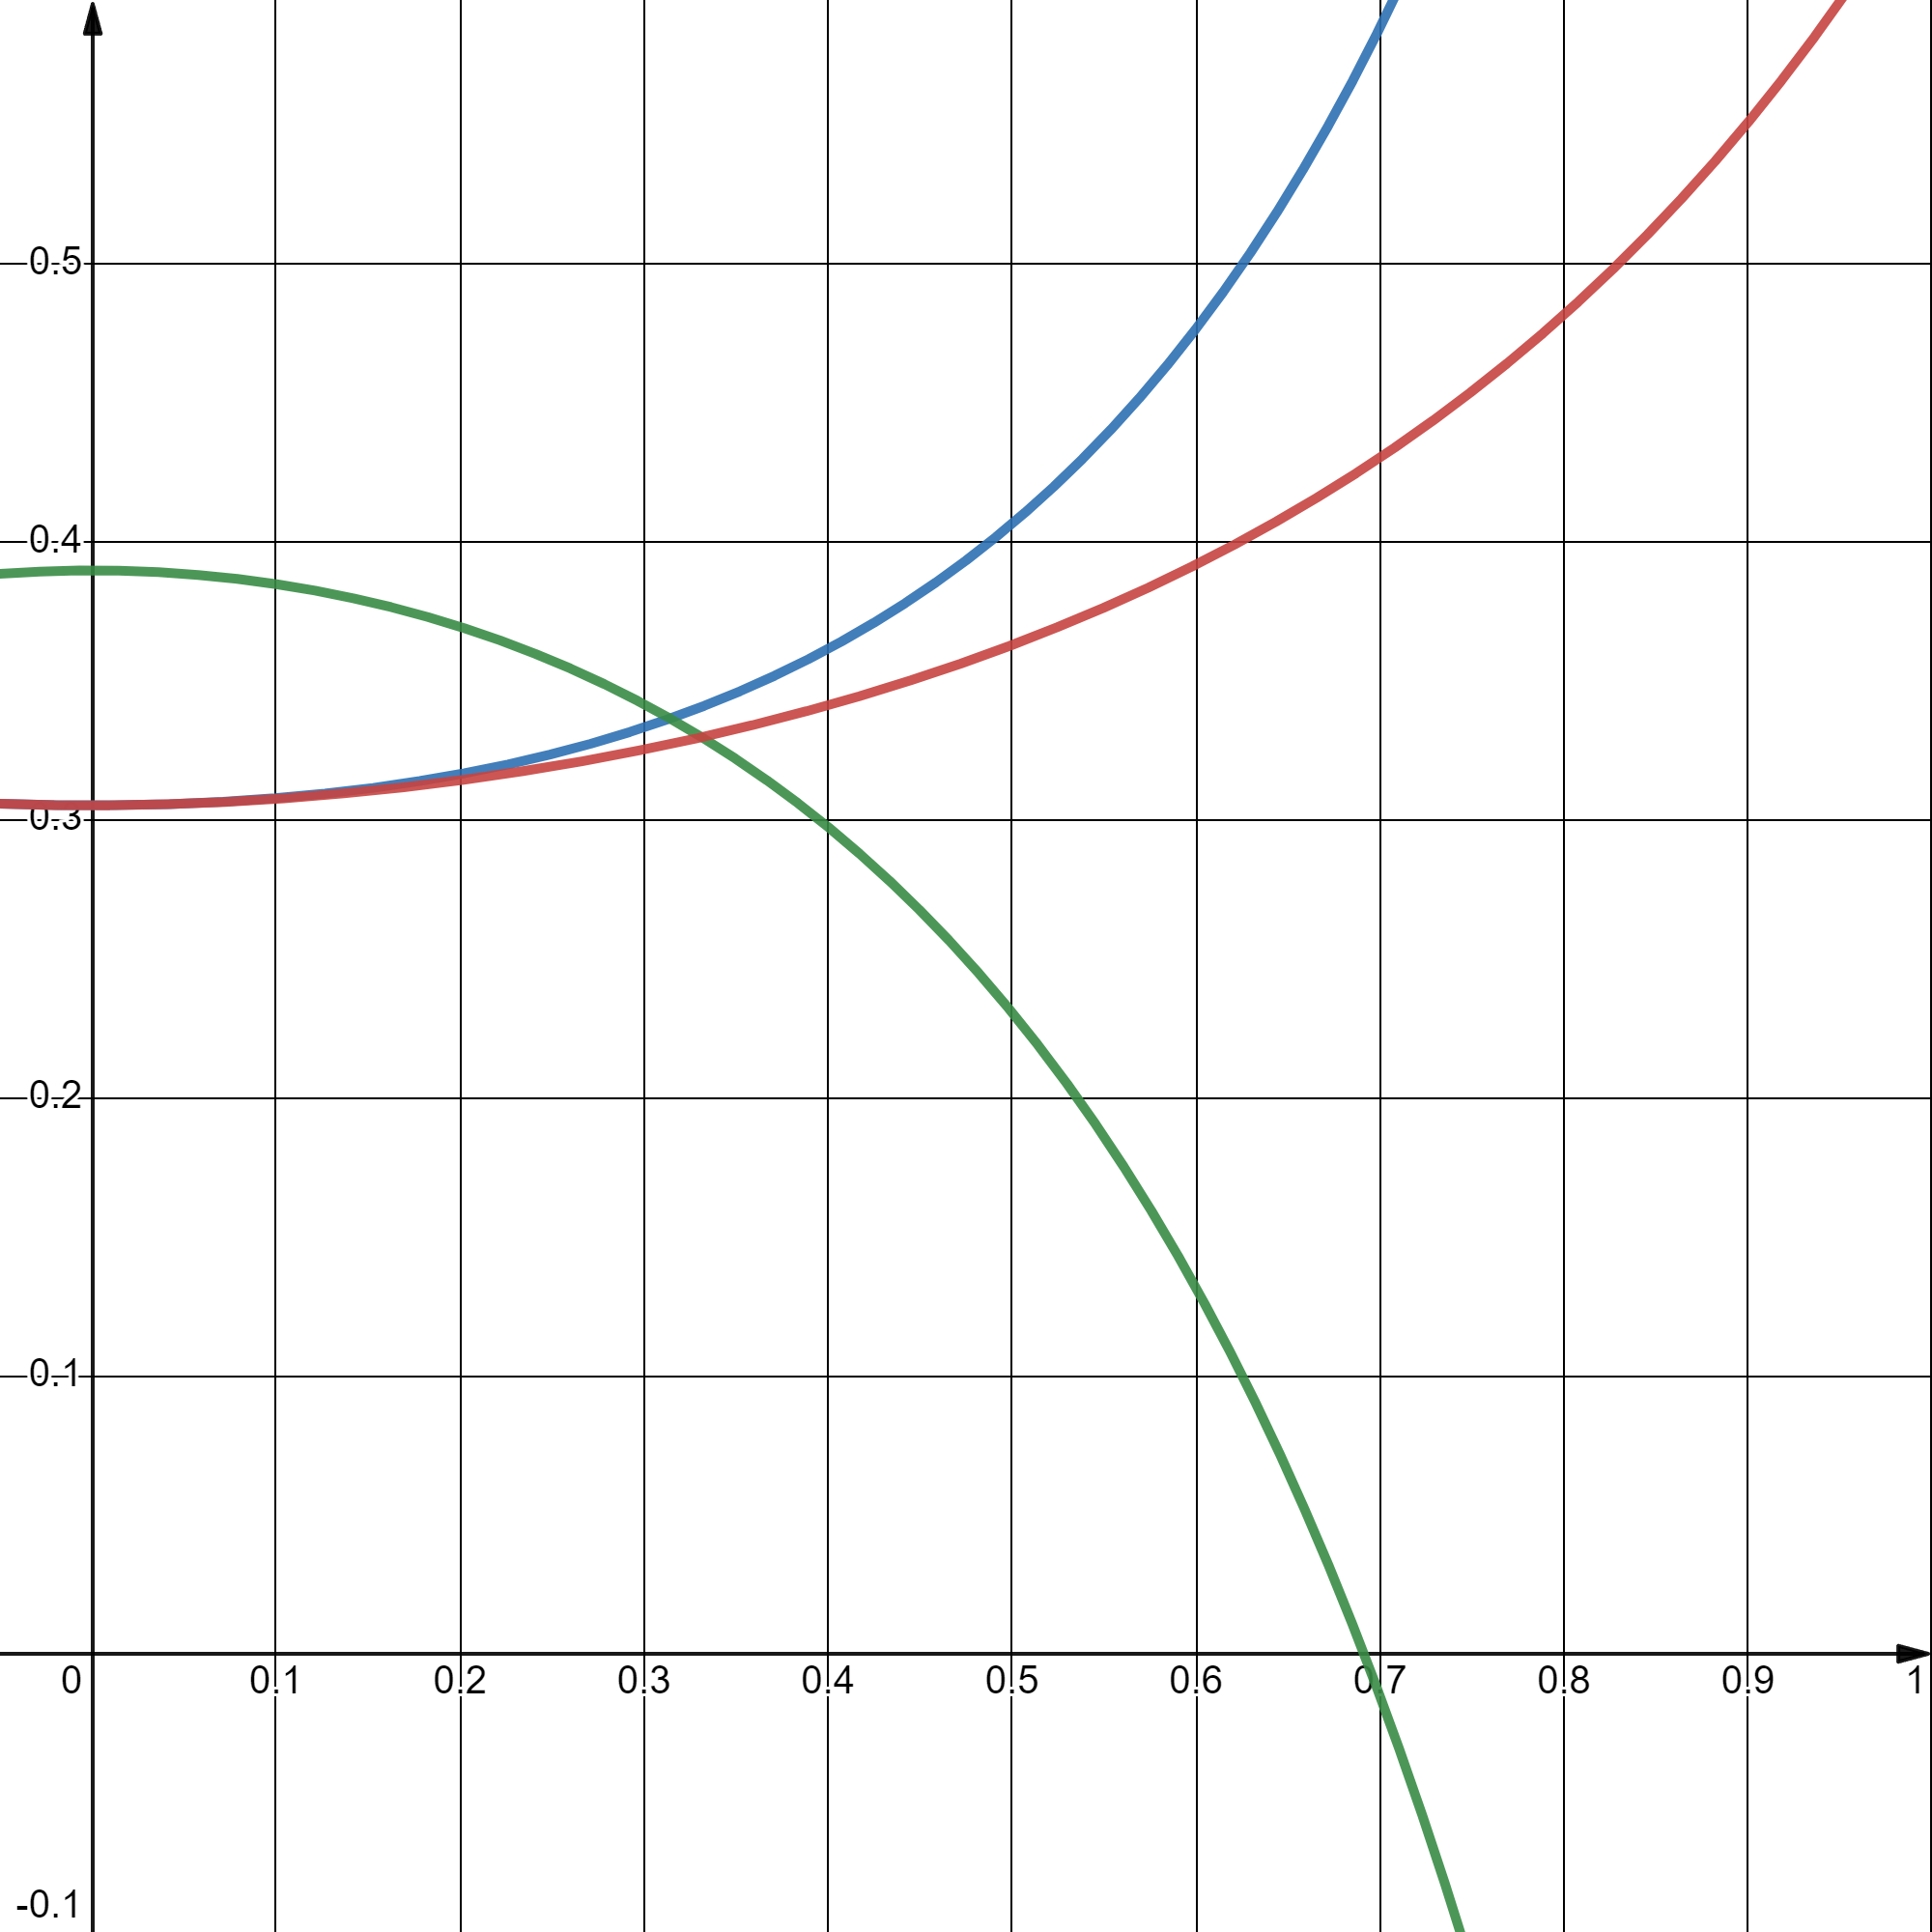
\includegraphics[scale=0.08]{prob.png}
	\end{center}
	
	$p_{2}\geq$ при $\sigma\leq 0.6913$. Вероятности $p_{1}$ и $p_{3}$ положительные при любом параметре $\sigma$.
	
	Получили условие $\sigma\leq 0.6913$.
	
\end{frame}

\begin{frame}{Варианты постановки задачи}
	\textbf{Задача:} имеются квантили $x_{\pi}$, $x_{0.5}$, $x_{1-\pi}$ логнормальной случайной величины $\eta$. Нужно уметь считать $m$ и $s^{2}$.
	
	\begin{enumerate}
		\item Используя значения двух квантилей, найти значения параметров $\mu$ и $\sigma$ нормальной случайной величины $\ln(\eta)\sim N(\mu, \sigma)$. Через них вычислить значения $m$ и $s^{2}$.
		\item Перейти к трехточечной аппроксимации дискретной случайной величиной $\xi_{n}$, у которой $m_{n} = m$ и $s^{2}=s^{2}$. И считать значения $m$ и $s$ через квантили $x_{\pi}$, $x_{0.5}$, $x_{1-\pi}$ и вероятности $p_{1}$, $p_{2}$, $p_{3}$.
		\item Если условие для положительных вероятностей не выполняется, можно воспринимать задачу не как поиск вероятностей для $\xi_{n}$, а как поиск коэффициентов для $x_{\pi}$, $x_{0.5}$, $x_{1-\pi}$ таких, чтобы параметры, посчитанные как мат.ожидание и дисперсия, были равны $m$ и $s^{2}$. 
	\end{enumerate}
\end{frame}

\begin{frame}{Точность аппроксимации мат.ожидания}
	\textbf{Проблема:} правило 30-40-30 используют для логнормального распределения.
	
	\textbf{Вопрос:} какова точность аппроксимации $m$ и $s^{2}$?
	
	\begin{proposition}\label{pr5}
		Ошибка аппроксимации мат.ожидания логнормального распределения с помощью правила 30-40-30 равна
		\[\dfrac{\mid m - \widetilde{m} \mid}{m} = \mid \exp(\dfrac{\sigma^{2}}{2}) - \dfrac{1}{2(\Phi^{-1}(0.1))^{2}}\times\]\[\times(\exp(\sigma\Phi^{-1}(0.1))-1 +\exp(\sigma\Phi^{-1}(0.9))) + 1 \mid/\exp\left(\dfrac{\sigma^{2}}{2}\right)\]
		и не зависит от параметра $\mu$.
	\end{proposition}
	\textit{\textbf{Доказательство:}}
		Выразим ошибку аппроксимации через параметры $\mu$ и $\sigma$.
\end{frame}

\begin{frame}{Точность аппроксимации мат.ожидания}
	\[m = \exp\left(\mu+\dfrac{\sigma^{2}}{2}\right).\]
	Имеем следующие квантили
	\[x_{\pi} = \exp(\mu+\sigma\Phi^{-1}(0.1)),\]
	Точные значения вероятностей
	\[p_{1} = p_{3} = \dfrac{1}{2(\Phi^{-1}(0.1))^{2}},\]
	\[p_{2} = 1 - \dfrac{1}{(\Phi^{-1}(0.1))^{2}}.\]
	
	Получили ошибку
	\[\dfrac{\mid m - \widetilde{m} \mid}{m} = \mid \exp(\dfrac{\sigma^{2}}{2}) - \dfrac{1}{2(\Phi^{-1}(0.1))^{2}}\times\]\[\times(\exp(\sigma\Phi^{-1}(0.1))-1 +\exp(\sigma\Phi^{-1}(0.9))) + 1 \mid/\exp\left(\dfrac{\sigma^{2}}{2}\right)\]
\end{frame}

\begin{frame}{Точность аппроксимации мат.ожидания}
	
	Построим график зависимости от $\sigma$.
	
	\begin{figure}[h]
		\begin{minipage}[h]{0.4\linewidth}
			\center{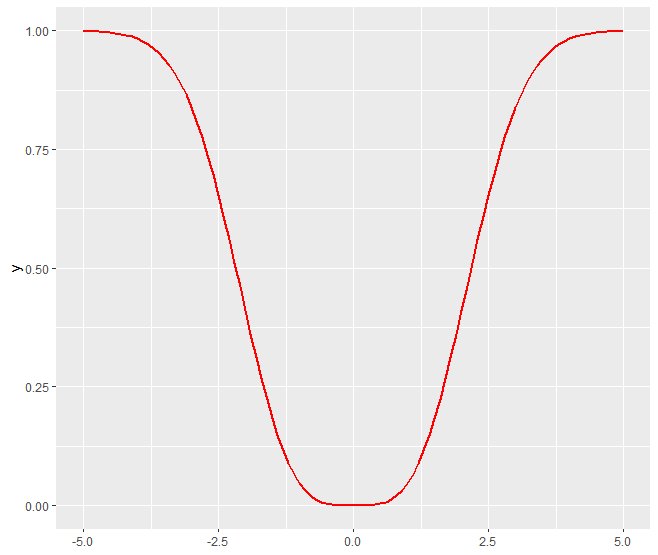
\includegraphics[width=1\linewidth]{ris1.png} \\}
		\end{minipage}
		\hfill
		\begin{minipage}[h]{0.4\linewidth}
			\center{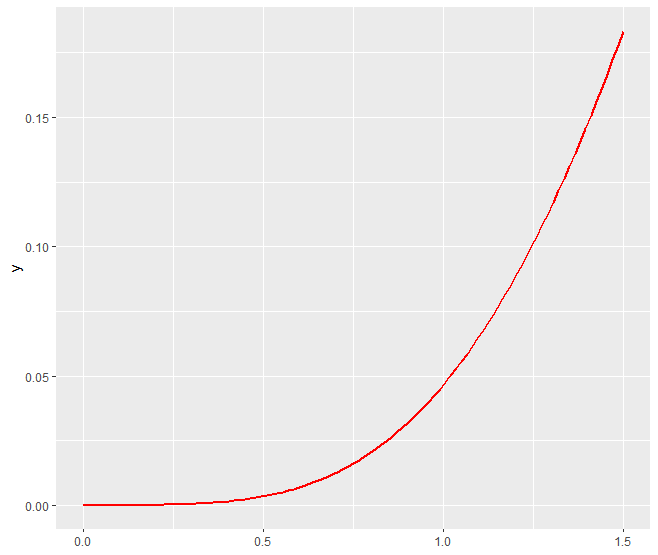
\includegraphics[width=1\linewidth]{ris2.png} \\}
		\end{minipage}
		\caption{Ошибка аппроксимации мат.ожидания}
		\label{ris:image1}
	\end{figure}
	
	Видим, что при $\sigma\leq1.5$ ошибка аппроксимации мат.ожидания меньше $12\%$. 
	
\end{frame}

\begin{frame}{Точность аппроксимации дисперсии}
	\begin{proposition}\label{pr6}
		Ошибка аппроксимации дисперсии логнормального распределения с помощью правила 30-40-30 равна
		\[\dfrac{\mid d - \widetilde{d} \mid}{d} = \mid \exp(\sigma^{2})(\exp(\sigma^{2}-1)) -\]\[- \dfrac{1}{2(\Phi^{-1}(0.1))^{2}}\exp(2\sigma\Phi^{-1}(0.1))-\]
		\[- \left(1 - \dfrac{1}{(\Phi^{-1}(0.1))^{2}}\right)\exp(2\sigma\Phi^{-1}(0.5))-\]
		\[-\dfrac{1}{2(\Phi^{-1}(0.1))^{2}}\exp(2\sigma\Phi^{-1}(0.9)) + m_{2}^{2}/2\mu\mid/\exp(\sigma^{2})(\exp(\sigma^{2}-1))\]
		
		и не зависит от параметра $\mu$.
	\end{proposition}
\end{frame}
\begin{frame}{Точность аппроксимации дисперсии}
	
	\textit{\textbf{Доказательство:}}
	Имеем ошибку
	\[\dfrac{\mid d - \widetilde{d} \mid}{d} = \mid \exp(2\mu+\sigma^{2})(\exp(\sigma^{2}-1)) -\]\[- \dfrac{1}{2(\Phi^{-1}(0.1))^{2}}\exp(2\mu+2\sigma\Phi^{-1}(0.1))-\]\[-
	 \left(1 - \dfrac{1}{(\Phi^{-1}(0.1))^{2}}\right)\exp(2\mu+2\sigma\Phi^{-1}(0.5))-\]
	\[-\dfrac{1}{2(\Phi^{-1}(0.1))^{2}}\exp(2\mu+2\sigma\Phi^{-1}(0.9)) + m_{2}^{2}\mid/\exp(2\mu+\sigma^{2})(\exp(\sigma^{2}-1))\]
	\[=\mid \exp(\sigma^{2})(\exp(\sigma^{2}-1)) - \dfrac{1}{2(\Phi^{-1}(0.1))^{2}}\exp(2\sigma\Phi^{-1}(0.1))-\]
	\[- \left(1 - \dfrac{1}{(\Phi^{-1}(0.1))^{2}}\right)\exp(2\sigma\Phi^{-1}(0.5))-\]
	\[-\dfrac{1}{2(\Phi^{-1}(0.1))^{2}}\exp(2\sigma\Phi^{-1}(0.9)) + m_{2}^{2}/2\mu\mid/\exp(\sigma^{2})(\exp(\sigma^{2}-1)).\]
	
\end{frame}

\begin{frame}{Точность аппроксимации дисперсии}
	
Построим график зависимости от $\sigma$.

\begin{figure}[h]
	\begin{minipage}[h]{0.4\linewidth}
		\center{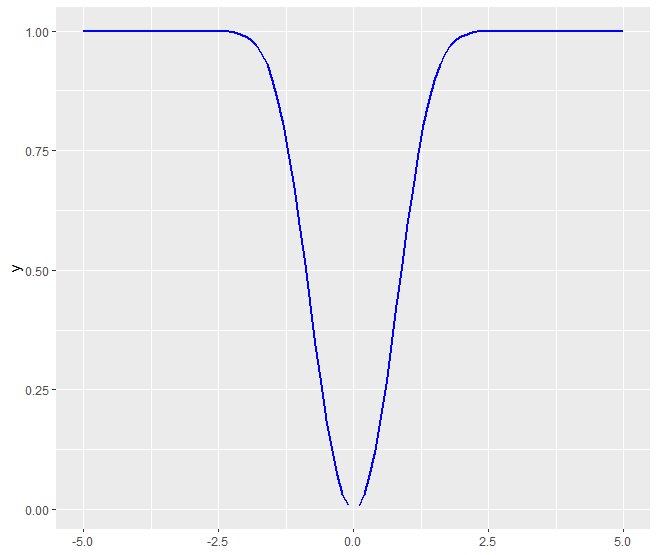
\includegraphics[width=1\linewidth]{ris3.png} \\}
	\end{minipage}
	\hfill
	\begin{minipage}[h]{0.4\linewidth}
		\center{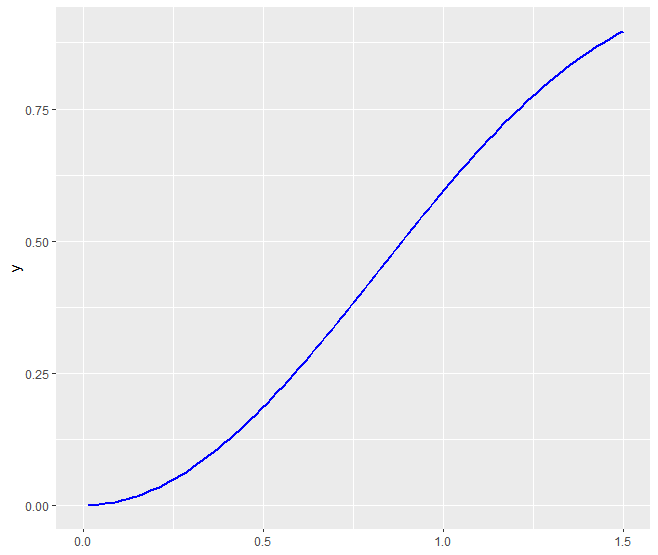
\includegraphics[width=1\linewidth]{ris4.png} \\}
	\end{minipage}
	\caption{Ошибка аппроксимации дисперсии}
	\label{figCurves}
\end{figure}

Видим, что при $\sigma\leq1.5$ ошибка аппроксимации дисперсии может достигать $80\%$. 
	
\end{frame}
	
	\begin{frame}{Произведение двух логнормальных распределений}
		Рассмотрим две логнормально распределенные случайные величины.
		\begin{itemize}
			\item $\ln(\xi_{1}) \sim N(\mu_{1}, \sigma _{1}^{2})$.
			\item $\ln(\xi_{2}) \sim N(\mu_{2}, \sigma _{2}^{2})$.
		\end{itemize}
		
		\textbf{Задача:} замена непрерывной случайной величины, полученной с помощью произведения двух логнормально распределенных случайных величин, дискретной. То есть записать произведение в виде дискретной аппроксимации с кванилями того же вида.
		
		\begin{itemize}
			\item $x_{\pi}$, $x_{0.5}$, $x_{1-\pi}$ "--- симметричные квантили $\xi_{1}$,
			\item $y_{\pi}$, $y_{0.5}$, $y_{1-\pi}$ "--- симметричные квантили $\xi_{2}$.
		\end{itemize}
		
	\end{frame}
	
	\begin{frame}{Произведение $\pi$-ых квантилей}
		\begin{proposition}
			При перемножении квантилей $x_{\pi}$ и $y_{\pi}$ двух логнормальных случайных величин $\xi_{1}$ и $\xi_{2}$ получается квантиль случайной величины $\xi_{1}\xi_{2}$ вида $z_{q}$, где
			
			
				\[q = \mathsf{P}(\xi_{1}\xi_{2}< x_{\pi}y_{\pi})=\]\[= \Phi\left(\frac{\Phi^{-1}(\pi)(\ln(x_{0.5})+\ln(y_{0.5})-\ln(x_{\pi})-\ln(y_{\pi}))}{\sqrt{(\ln(x_{0.5})-\ln(x_{\pi}))^{2}+(\ln(y_{0.5})-\ln(y_{\pi}))^{2}}}\right).\]
			
		\end{proposition}
	\textbf{\textit{Доказательство:}}
	Выразим параметры распределений $\mu_{1}$, $\mu_{2}$, $\sigma_{1}$, $\sigma_{2}$ через квантили.
	\begin{equation*}
		\mathsf{P}(\xi_{1}<x_{\pi}) = \mathsf{P}(\ln(\xi_{1})<\ln(x_{\pi})) = \mathsf{P}\left(\dfrac{\ln(\xi_{1})-\mu_{1}}{\sigma_{1}} < \frac{\ln(x_{\pi})-\mu_{1}}{\sigma_{1}}\right).
	\end{equation*}
	 \[\dfrac{\ln(\xi_{1})-\mu_{1}}{\sigma_{1}} \sim N(0,1).\]
	
	\end{frame}
	
	\begin{frame}{Произведение $\pi$-ых квантилей}
		
		\begin{equation*}
			\ln(x_{\pi})=\sigma_{1}\Phi^{-1}(\pi)+\mu_{1}.\label{12}
		\end{equation*}

		\begin{equation*}
			\mu_{1}=\ln(x_{0.5}).\label{13}
		\end{equation*}
		\begin{equation*}
			\sigma_{1}=\frac{\ln(x_{\pi})-\ln(x_{0.5})}{\Phi^{-1}(\pi)}.\label{14}
		\end{equation*}
		\begin{equation*}
			\frac{\ln(y_{\pi})-\mu_{2}}{\sigma_{2}}=\Phi^{-1}(\pi),\label{15}
		\end{equation*}
		\begin{equation*}
			\mu_{2}=\ln(y_{0.5}).\label{16}
		\end{equation*}

		\begin{equation*}
			\displaystyle{\sigma_{2}=\frac{\ln(y_{\pi})-\ln(y_{0.5})}{\Phi^{-1}(\pi)}.\label{17}}
		\end{equation*}
		
		Рассмотрим случайную величину $\eta = \xi_{1}\xi_{2}$. Нужно вычислить, каким квантилем для $\eta$ является произведение квантилей $x_{\pi}$ и $y_{\pi}$. 
		
		Для этого надо найти, чему равна вероятность $\mathsf{P}(\xi_{1}\xi_{2}< x_{\pi}y_{\pi})$.
		
	\end{frame}
	
	\begin{frame}{Произведение $\pi$-ых квантилей}
		
		\begin{equation*}
			\mathsf{P}(\xi_{1}\xi_{2}< x_{\pi}y_{\pi}) = \mathsf{P}(\ln(\xi_{1})+\ln(\xi_{2})<\ln(x_{\pi})+\ln(y_{\pi}))=
		\end{equation*}
		\begin{equation*}
			=\mathsf{P}\left(\displaystyle{\frac{\ln(\xi_{1})+\ln(\xi_{2})-(\mu_{1}+\mu_{2})}{\sqrt{\sigma_{1}^{2}+\sigma_{2}^{2}}}}<\displaystyle{\frac{\ln(x_{\pi})+\ln(y_{\pi})-(\mu_{1}+\mu_{2})}{\sqrt{\sigma_{1}^{2}+\sigma_{2}^{2}}}}\right).
		\end{equation*}
		
		\begin{equation*} 
			\ln(\xi_{1})+\ln(\xi_{2})\sim N(\mu_{1}+\mu_{2}, \sigma_{1}^{2}+\sigma_{2}^{2}),
		\end{equation*}
		\begin{equation*}
			\frac{\ln(\xi_{1})+\ln(\xi_{2})-(\mu_{1}+\mu_{2})}{\sqrt{\sigma_{1}^{2}+\sigma_{2}^{2}}} \sim N(0,1).
		\end{equation*}
		\begin{equation*}
			\ln(x_{\pi})=\mu_{1}+\Phi^{-1}(\pi)\sigma_{1},
		\end{equation*}
		\begin{equation*}
			\ln(y_{\pi})=\mu_{2}+\Phi^{-1}(\pi)\sigma_{2}.
		\end{equation*}
	
		\begin{equation*}
			\mathsf{P}(\xi_{1}\xi_{2}< x_{\pi}y_{\pi}) =
		\end{equation*}
		\begin{equation*}
			=\Phi\left(\frac{\Phi^{-1}(\pi)(\sigma_{1}+\sigma_{2})}{\sqrt{\sigma_{1}^{2}+\sigma_{2}^{2}}}\right).
		\end{equation*}
	
	\end{frame}
	\begin{frame}{Произведение $\pi$-ых квантилей}
		
			\[\frac{\Phi^{-1}(\pi)(\sigma_{1}+\sigma_{2})}{\sqrt{\sigma_{1}^{2}+\sigma_{2}^{2}}}=\]\[=
			\dfrac{(\ln(x_{0.5})-\ln(x_{\pi}))+(\ln(y_{0.5})-\ln(y_{\pi}))}{\dfrac{\sqrt{(\ln(x_{0.5})-\ln(x_{\pi}))^{2}+(\ln(y_{0.5})-\ln(y_{\pi}))^{2}}}{\Phi^{-1}(\pi)}}.\]
		
		
		Тогда получаем следующую формулу
		\begin{equation*}
			\mathsf{P}(\xi_{1}\xi_{2}< x_{\pi}y_{\pi}) =\Phi\left(\frac{\Phi^{-1}(\pi)(\ln(x_{0.5})+\ln(y_{0.5})-\ln(x_{\pi})-\ln(y_{\pi}))}{\sqrt{(\ln(x_{0.5})-\ln(x_{\pi}))^{2}+(\ln(y_{0.5})-\ln(y_{\pi}))^{2}}}\right).
		\end{equation*}
	\end{frame}

	\begin{frame}{Квантили вида $\pi$, 0.5, $1-\pi$}
	
		\begin{proposition}
		Зная квантили $x_{\pi}$, $x_{0.5}$, $x_{1-\pi}$ случайной величины $\xi_{1}$ и квантили $y_{\pi}$, $y_{0.5}$, $y_{1-\pi}$ случайной величины $\xi_{2}$ можно найти квантили $z_{\pi}$, $z_{0.5}$, $z_{1-\pi}$ случайной величины $\xi_{1}\xi_{2}$, как
		
		\begin{equation*}
			z_{\pi}=\exp(\sigma\Phi^{-1}(\pi)+a),
		\end{equation*}
		\begin{equation*}
			z_{0.5}=x_{0.5}y_{5},
		\end{equation*}
		\begin{equation*}
			z_{1-\pi}=\exp(\sigma\Phi^{-1}(1-\pi)+a),
		\end{equation*}
		
		где $a$ и $\sigma$ -- параметры прямой $\dfrac{x-a}{\sigma}$, на которой лежат точки $(\ln(x_{\pi}y_{\pi}), t)$ и $(\ln(x_{0.5}y_{0.5}),0)$,
		\begin{equation*}
			t = \frac{\Phi^{-1}(\pi)((\ln(x_{0.5})+\ln(y_{0.5}))-(\ln(x_{\pi})+\ln(y_{\pi})))}{\sqrt{(\ln(x_{0.5})-\ln(x_{\pi}))^{2}+(\ln(y_{0.5})-\ln(y_{\pi}))^{2}}}. 
		\end{equation*}
	\end{proposition}
\end{frame}

\begin{frame}{Квантили вида $\pi$, 0.5, $1-\pi$}
	\textbf{\textit{Доказательство:}}
	С помощью формулы (18) можно посчитать, какой получается квантиль для случайной величины $\xi_{1}\xi_{2}$, если перемножить квантили $x_{\pi}$ и $y_{\pi}$ исходных случайных величин.
	
	\begin{equation*}
		\mathsf{P}(\xi_{1} \xi_{2} < x_{0.5}y_{0.5}) = \Phi(0) = 0.5.
	\end{equation*}
	Получили снова 0.5-ый квантиль. 
	
	Обозначим $z_{\pi}$, $z_{0.5}$, $z_{1-\pi}$ "--- квантили случайной величины $\eta$.
	Тогда $x_{0.5}y_{0.5} = z_{0.5}$.
	
	C помощью точек $(\ln(x_{\pi}y_{\pi}), t)$ и $(\ln(x_{0.5}y_{0.5}),0)$  можно найти параметры $a$ и $\sigma$ прямой, на которой они лежат.
	\begin{equation*}
		\dfrac{\ln(x_{0.5}y_{0.5})-a}{\sigma}=0 \quad\quad \Rightarrow \quad\quad a=\ln(x_{0.5}y_{0.5}),
	\end{equation*}
	
\end{frame}

\begin{frame}{Квантили вида $\pi$, 0.5, $1-\pi$}
	
	\begin{equation*}
		\dfrac{\ln(x_{\pi}y_{\pi})-a}{\sigma}=t,
	\end{equation*}
	
	\begin{equation*}
		\sigma=\dfrac{\ln(x_{\pi}y_{\pi})-a}{t}=\dfrac{\ln(x_{\pi}y_{\pi})-\ln(x_{0.5}y_{0.5})}{t}.
	\end{equation*}

Так как точки $(\ln(z_{\pi}), \Phi^{-1}(\pi))$ и $(\ln(z_{1-\pi}), \Phi^{-1}(1-\pi))$ тоже лежат на этой прямой, то мы можем вычислить значения $\ln(z_{\pi})$ и $\ln(z_{0.5})$, зная уравнение прямой, следующим образом:
\begin{equation*}
	\dfrac{\ln(z_{\pi})-a}{\sigma}=\Phi^{-1}(\pi),
\end{equation*}
\begin{equation*}
	\ln(z_{\pi})=\sigma\Phi^{-1}(\pi)+a,
\end{equation*}

\begin{equation*}
	\dfrac{\ln(z_{1-\pi})-a}{\sigma}=\Phi^{-1}(1-\pi),
\end{equation*}
\begin{equation*}
	\ln(z_{1-\pi})=\sigma\Phi^{-1}(1-\pi)+a.
\end{equation*}

И, наконец, находим $z_{\pi}$ и $z_{1-\pi}$.
\begin{equation*}
	z_{\pi}=\exp(\sigma\Phi^{-1}(\pi)+a),
\end{equation*}
\begin{equation*}
	z_{1-\pi}=\exp(\sigma\Phi^{-1}(1-\pi)+a).
\end{equation*}
	
\end{frame}

\begin{frame}{Сумма двух логнормальных распределений }
	
		Рассмотрим сумму двух логнормальных случайных величин.
	\begin{equation*}
		\ln(\xi_{1}) \sim N(\mu_{1}, \sigma _{1}^{2}),
	\end{equation*}
	\begin{equation*}
		\ln(\xi_{2}) \sim N(\mu_{2}, \sigma _{2}^{2}),
	\end{equation*}
	\begin{equation*}
		\eta = \xi_{1}+\xi_{2}.
	\end{equation*}
	
	\textbf{Задача:} найти квантили $z_{\pi}$, $z_{0.5}$, $z_{1-\pi}$ случайной величины $\eta$, а также вычислить вероятности $p_{1}$, $p_{2}$, $p_{3}$ такие, что $m = m_{n}$  и $s^{2} = s^{2}_{n}$.
	
	Чтобы найти $z_{10}$, $z_{50}$, $z_{90}$ будем использовать аппроксимацию суммы логнормальных распределений логнормальным распределением. $\ln(\eta)\sim N(\mu, \sigma)$.
	
	\textbf{Альтернатива:}
	Если это ограничение на $\sigma$ не выполняется и мы не можем вычислить положительные вероятности, то можно не переходить к аппроксимации дискретным распределением, а вычислить значения мат. ожидания и дисперсии $\eta$ с помощью квантилей $z_{\pi}$, $z_{0.5}$, $z_{1-\pi}$.
	
\end{frame}

\begin{frame}{Сумма двух логнормальных распределений }
	
	\begin{pr1}
		Квантили $x_{\pi}$, $x_{0.5}$, $x_{1-\pi}$ "--- квантили $\xi_{1}$, $y_{\pi}$, $y_{0.5}$, $y_{1-\pi}$ "--- квантили $\xi_{2}$.
	\end{pr1}
	\begin{enumerate}
		\item Найти параметры $\mu_{1}$, $\sigma_{1}$, $\mu_{2}$ и $\sigma_{2}$ через значения квантилей, используя формулы раздела 4.2.
		\item Вычислить значения мат. ожидания $m$ и дисперсии $s^{2}$ случайной величины $\xi_{1} + \xi_{2}$, как суммы $m = m_{1}+m_{2}$, $d=d_{1} + d_{2}$, где $m_{1}, d_{1}$ -- мат.ожидание и дисперсия $\xi_{1}$, а $m_{2}$, $d_{2}$ -- случайной величины $\xi_{2}$. Они пересчитываются аналогично $m$ и $d$.
		\item Выразить параметры $\mu$ и $\sigma$ нормального распределения через параметры $m$ и $d$ логнормального распределения.
		
	\end{enumerate}
	
	
	
\end{frame}
	
\begin{frame}{Сумма двух логнормальных распределений }
	

	\begin{enumerate}
		\item Вычислить, какой квантиль получается при сложении $x_{\pi}$ и $y_{\pi}$, используя следующую формулу
		
		\begin{equation*}
			\mathsf{P}(\xi_{1}+\xi_{2}< x_{\pi}+y_{\pi}) = \mathsf{P}(\ln(\xi_{1}+\xi_{2})<\ln(x_{\pi}+y_{\pi}))=
		\end{equation*}
		
		
			\[=\mathsf{P}\left(\displaystyle{\frac{\ln(\xi_{1}+\xi_{2})-\mu}{\sigma}}<\displaystyle{\frac{\ln(x_{\pi}+y_{\pi})-\mu}{\sigma}}\right)=\]\[ =\Phi\left(\dfrac{\ln(x_{\pi}+y_{\pi})-\mu}{\sigma}\right).\]
		
		
		\item Найти значения квантилей $z_{10}$, $z_{50}$, $z_{90}$ по Алгоритму 2.
	\end{enumerate}
	\begin{pr3}\end{pr3} вероятности $p_{1}$, $p_{2}$, $p_{3}$ для $z_{\pi_{1}}, z_{\pi_{2}}, z_{\pi_{3}}$ случайной величины $\xi_{1} + \xi_{2}$.
	
	
\end{frame}

\begin{frame}{Точность аппроксимации }
	
	Oшибки аппроксимации квантилей $q_{10}$, $q_{50}$, $q_{90}$ случайной величины $\eta$ равны
\[\dfrac{\left| q_{10} - z_{10}\right|}{q_{10}}, \quad\quad \dfrac{\left| q_{50} - z_{50}\right|}{q_{50}}, \quad\quad \dfrac{\left| q_{90} - z_{90}\right|}{q_{90}},\] где
\[z_{p*100} = F_{\eta_{n}}^{-1}(p) = \exp(\mu+\sigma\sqrt{2}\mathrm{erf}^{-1}(2p-1)).\]
Значение квантилей $q_{i}$ выражаются как $q_{p*100} = F_{\eta}^{-1}(p)$, где
\[F_{\eta}(x) = \int_{0}^{x}\left( \dfrac{1}{2}+\dfrac{1}{2} \mathrm{erf}\left( \dfrac{\ln(x-y)-\mu_{1}}{\sigma_{1}\sqrt{2}}\right) \right)\times\]
\[\times \left( \dfrac{1}{\sqrt{2\pi}y\sigma_{2}}\exp\left( -\left( \dfrac{\ln(y)-\mu_{2}}{\sqrt{2}\sigma_{2}}\right) ^{2}\right) \right) dy \]
	
\end{frame}

\begin{frame}{Точность аппроксимации }
	Рассмотрим $\ln(\xi_{1}) \sim N(4, \sigma _{1}^{2})$, $\ln(\xi_{2}) \sim N(6, \sigma _{1}^{2})$ и найдем ошибки с помощью моделирования.
	
	\bigskip
	
	Ниже приведены фрагменты таблиц с ошибками, выраженными в $\%$ для 0.05 < $\sigma_{1}^{2}, \sigma_{2}^{2}$ < 2.25.
	
	\begin{table}[ht]
		\centering
		\caption{Ошибка аппроксимации медианы  }
		\begin{tabular}{rrrrrr}
			\hline
			& \textbf{0.25} & \textbf{0.75} & \textbf{1.25} & \textbf{1.75} & \textbf{2.5} \\ 
			\hline
			\textbf{0.25} & 0.58 & 0.29 & 0.89 & 2.64 & 6.41 \\ 
			\textbf{0.75} & 0.13 & 0.12 & 2.15 & 4.88 & 7.27 \\ 
			\textbf{1.25} & 0.01 & 0.83 & 2.94 & 5.58 & 10.02 \\ 
			\textbf{1.75} & 2.23 & 0.52 & 3.61 & 6.74 & 9.84 \\ 
			\textbf{2.5} & 9.15 & 3.35 & 3.25 & 6.76 & 9.89 \\ 
			\hline
		\end{tabular}
	\end{table}
	
\end{frame}

\begin{frame}{Точность аппроксимации }
	\begin{table}[ht]
		\centering
		\caption{Ошибка аппроксимации $q_{10}$ }
		\begin{tabular}{rrrrrr}
			\hline
			& \textbf{0.25} & \textbf{0.75} & \textbf{1.25} & \textbf{1.75} & \textbf{2.5} \\
			\hline
			\textbf{0.25} & 2.35 & 13.59 & 23.93 & 33.20 & 42.75 \\ 
			\textbf{0.75} & 1.20 & 10.54 & 21.80 & 33.93 & 42.82 \\ 
			\textbf{1.25} & 3.02 & 7.03 & 18.43 & 29.49 & 40.09 \\ 
			\textbf{1.75} & 14.45 & 5.27 & 14.33 & 26.50 & 36.75 \\ 
			\textbf{2.5} & 34.70 & 11.44 & 11.10 & 23.05 & 32.84 \\ 
			\hline
		\end{tabular}
	\end{table}
	
	\begin{table}[ht]
		\centering
		\caption{Ошибка аппроксимации $q_{90}$ }
		\begin{tabular}{rrrrrr}
			\hline
			& \textbf{0.25} & \textbf{0.75} & \textbf{1.25} & \textbf{1.75} & \textbf{2.5} \\
			\hline
			\textbf{0.25} & 1.01 & 3.00 & 4.24 & 4.10 & 3.40 \\ 
			\textbf{0.75} & 0.04 & 2.51 & 4.11 & 3.26 & 5.45 \\ 
			\textbf{1.25} & 1.44 & 1.81 & 3.29 & 3.93 & 5.82 \\ 
			\textbf{1.75} & 8.25 & 2.60 & 2.93 & 3.60 & 4.49 \\ 
			\textbf{2.5} & 18.17 & 3.00 & 3.30 & 2.44 & 4.99 \\ 
			\hline
		\end{tabular}
	\end{table}
	
\end{frame}

\begin{frame}{Точность аппроксимации }
	\begin{itemize}
		\item При аппроксимации суммы двух логнормальных распределений логнормальным распределением ошибки математического ожидания и дисперсии равны 0, то есть $m=m_{n}$ и $s^{2} = s_{n}^{2}$. Но ошибки аппроксимации квантилей $\eta$ могут достигать 11\% для $q_{50}$, ошибка  квантиля $q_{10}$ достигает 51\%, ошибка квантиля $q_{90}$ достигает 40\%.
		\bigskip
		\item При этом значения мат ожидания и дисперсии $\eta$, вычисленные по этим квантилям тоже имеют нулевую ошибку.
	\end{itemize}	
\end{frame}

\begin{frame}{Точность аппроксимации }
	Построим графики зависимости ошибки аппроксимации квантилей от $\sigma_{2}^{2}$ при фиксированной $\sigma_{1}^{2} = 0.45$. При моделировании объемы выборок равны $10^{6}$, а количество рассматриваемых $\sigma_{2}^{2}$ равно 23.
	\begin{figure}[h]
		\begin{center}
			\begin{minipage}[h]{0.45\linewidth}
				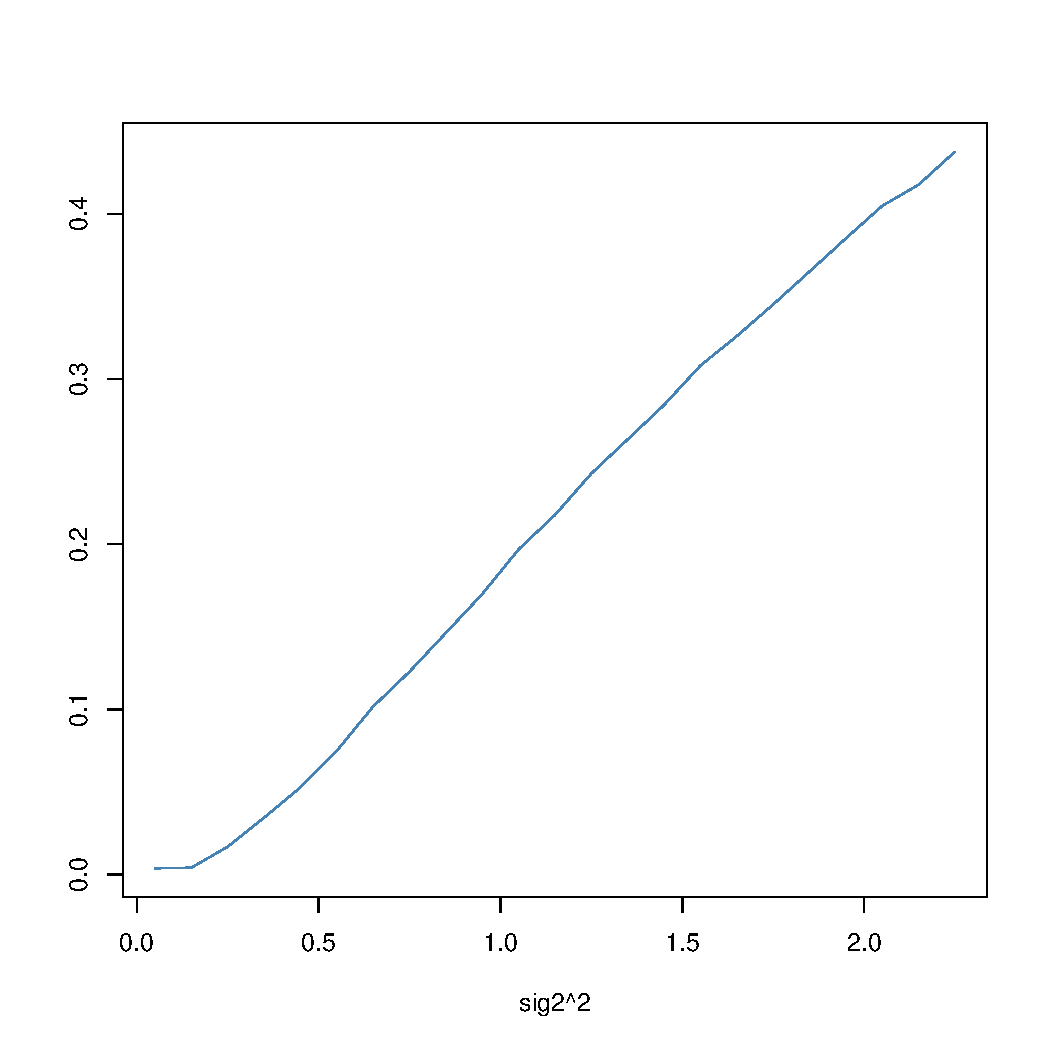
\includegraphics[width=1\linewidth]{gr_new_2.pdf}
				\caption{Ошибка аппроксимации $q_{10}$ при $\sigma_{1}^{2} = 0.45$.} %% подпись к рисунку
				\label{ris7} %% метка рисунка для ссылки на него
			\end{minipage}
		\end{center}
	\end{figure}	
\end{frame}

\begin{frame}{Точность аппроксимации }
	
	
	\begin{figure}[h]
		\begin{center}
			\begin{minipage}[h]{0.47\linewidth}
				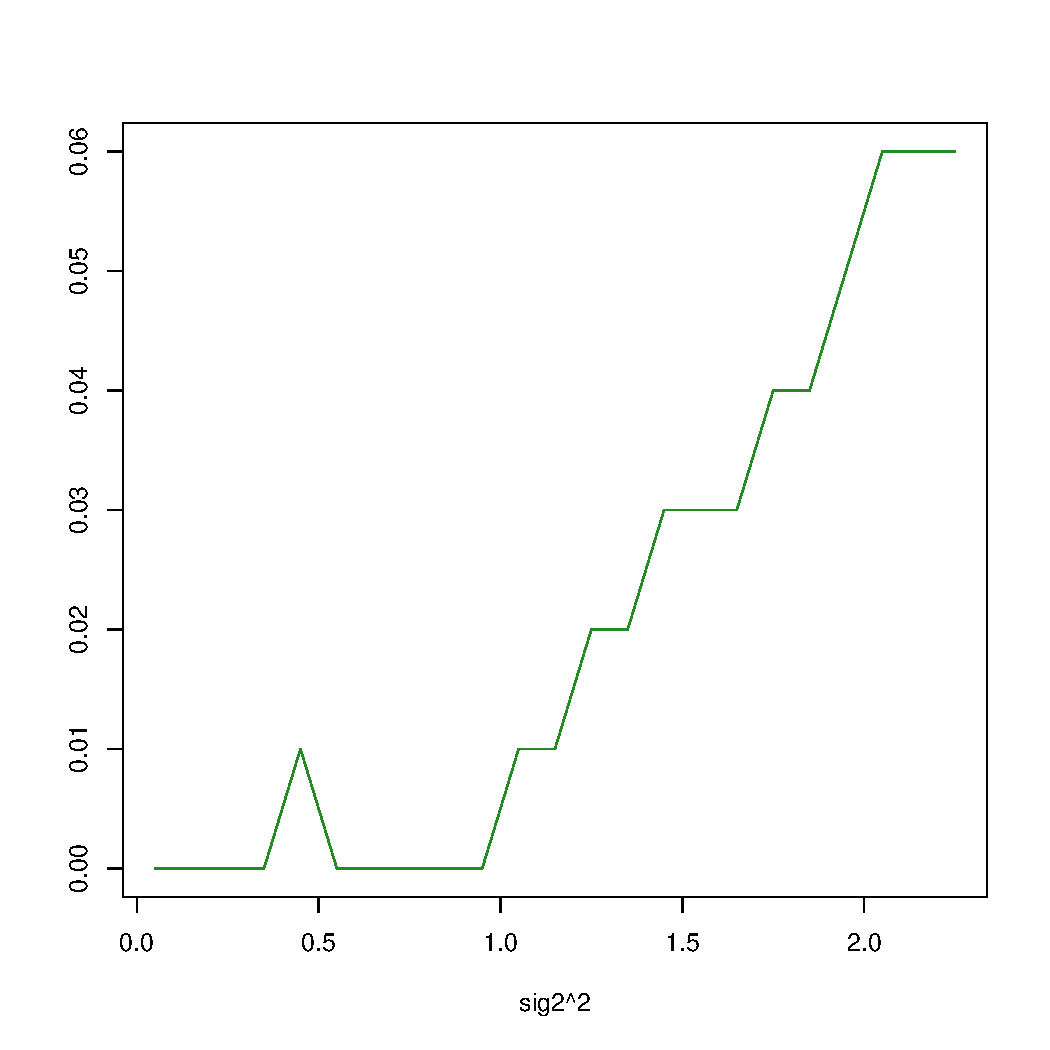
\includegraphics[width=1\linewidth]{gr_new_1.pdf}
				\caption{Ошибка аппроксимации медианы при $\sigma_{1}^{2} = 0.45$.} %% подпись к рисунку
				\label{ris7} %% метка рисунка для ссылки на него
			\end{minipage}
			\hfill
			\begin{minipage}[h]{0.47\linewidth}
				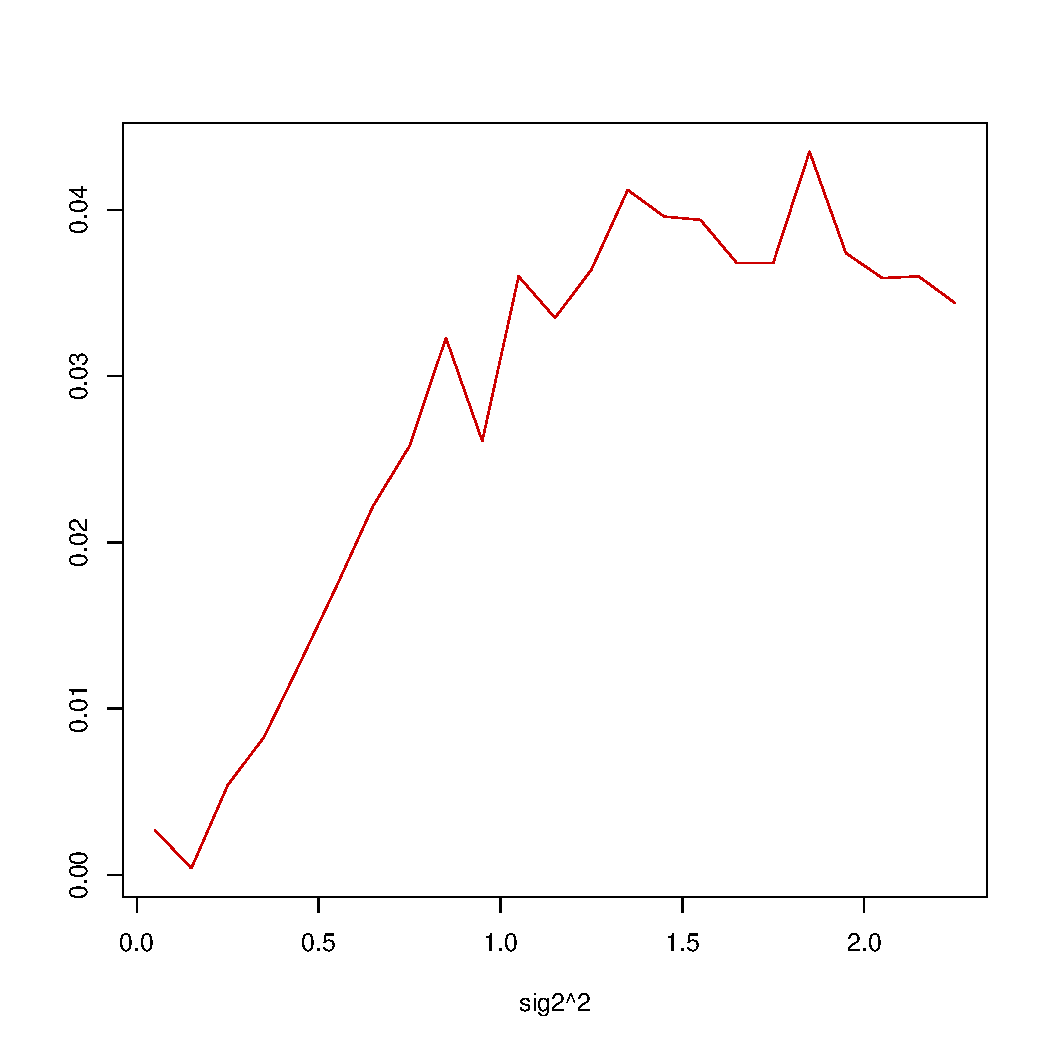
\includegraphics[width=1\linewidth]{gr_new_3.pdf}
				\caption{Ошибка аппроксимации $q_{90}$ при $\sigma_{1}^{2} = 0.45$.}
				\label{ris8}
			\end{minipage}

		\end{center}
	\end{figure}	
\end{frame}

\begin{frame}{Точность аппроксимации }
	
	Посчитаем значения функции $F_{\eta}(x)$ от квантилей $z_{10}$, $z_{50}$, $z_{90}$ случайной величины $\eta_{n}$ при 0.15 < $\sigma_{1}^{2}, \sigma_{2}^{2}$ < 2.25. Они показывают, каким квантилем для $\eta$ являются квантили $z_{i}$. Результаты приведены в следующих таблицаx.
	
	\begin{table}[!hhh]
		\centering
		\caption{$F_{\eta}(z_{50})$ в \% при 0.15 < $\sigma_{1}^{2}, \sigma_{2}^{2}$ < 2.25 }
		\label{tab4}
		\begin{tabular}{rrrrr}
			\hline
			& \textbf{0.15} & \textbf{0.85} & \textbf{1.55} & \textbf{2.25} \\
			\hline
			\textbf{0.15} & 0.51 & 0.50 & 0.49 & 0.48 \\ 
			\textbf{0.85} & 0.50 & 0.50 & 0.48 & 0.47 \\ 
			\textbf{1.55} & 0.49 & 0.50 & 0.48 & 0.46 \\ 
			\textbf{2.25} & 0.40 & 0.49 & 0.48 & 0.46 \\ 
			\hline
		\end{tabular}
	\end{table}	
\end{frame}

\begin{frame}{Точность аппроксимации }
	
	\begin{table}[!hhh]
		\centering
		\caption{$F_{\eta}(z_{10})$ при 0.15 < $\sigma_{1}^{2}, \sigma_{2}^{2}$ < 2.25 }
		\label{tab5}
		\begin{tabular}{rrrrr}
			\hline
			& \textbf{0.15} & \textbf{0.85} & \textbf{1.55} & \textbf{2.25} \\
			\hline
			\textbf{0.15} & 0.09 & 0.06 & 0.04 & 0.02 \\ 
			\textbf{0.85} & 0.10 & 0.07 & 0.05 & 0.03 \\ 
			\textbf{1.55} & 0.05 & 0.08 & 0.06 & 0.04 \\ 
			\textbf{2.25} & 0.00 & 0.08 & 0.07 & 0.05 \\ 
			\hline
		\end{tabular}
	\end{table}
	
	\begin{table}[!hhh]
		\centering
		\caption{$F_{\eta}(z_{90})$ при 0.15 < $\sigma_{1}^{2}, \sigma_{2}^{2}$ < 2.25 }
		\label{tab6}
		\begin{tabular}{rrrrr}
			\hline
			& \textbf{0.15} & \textbf{0.85} & \textbf{1.55} & \textbf{2.25} \\
			\hline
			\textbf{0.15} & 0.90 & 0.90 & 0.90 & 0.90 \\ 
			\textbf{0.85} & 0.90 & 0.91 & 0.91 & 0.90 \\ 
			\textbf{1.55} & 0.93 & 0.90 & 0.91 & 0.91 \\ 
			\textbf{2.25} & 0.95 & 0.91 & 0.90 & 0.91 \\ 
			\hline
		\end{tabular}
	\end{table}
\end{frame}

\begin{frame}{Точность аппроксимации }
	
	Также построим гистограммы для $\eta$ и $\eta_{n}$, когда ошибки имеют очень маленькие значения и когда достаточно большие.
	
	\begin{figure}[h]
		\begin{center}
			\begin{minipage}[h]{0.7\linewidth}
				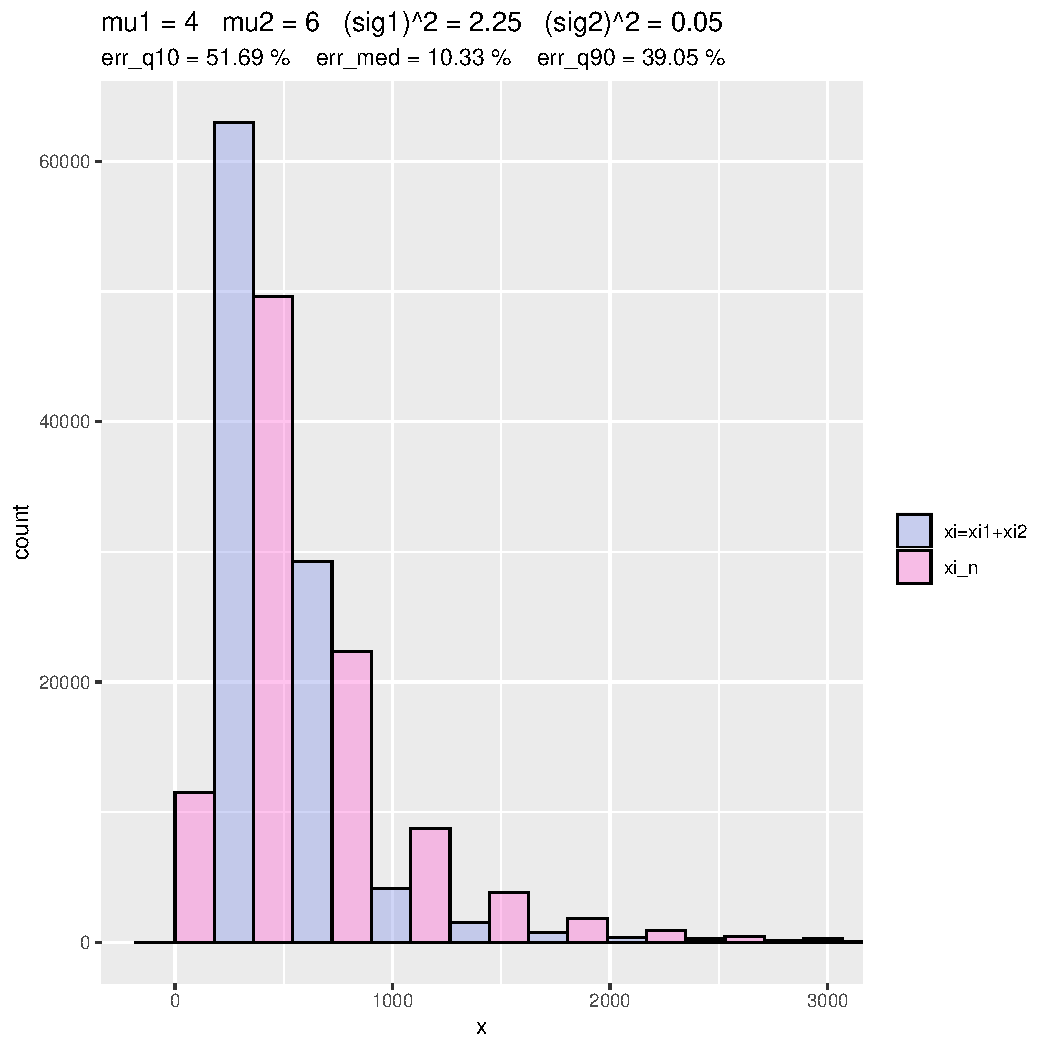
\includegraphics[width=1\linewidth]{hist_new_1.pdf}
				\caption{Сумма логнормальных.} %% подпись к рисунку
				\label{ris7} %% метка рисунка для ссылки на него
			\end{minipage}
			
		\end{center}
	\end{figure}	
	
\end{frame}

\begin{frame}{Точность аппроксимации }
	
	\begin{figure}[h]
		\begin{center}
			\begin{minipage}[h]{0.8\linewidth}
				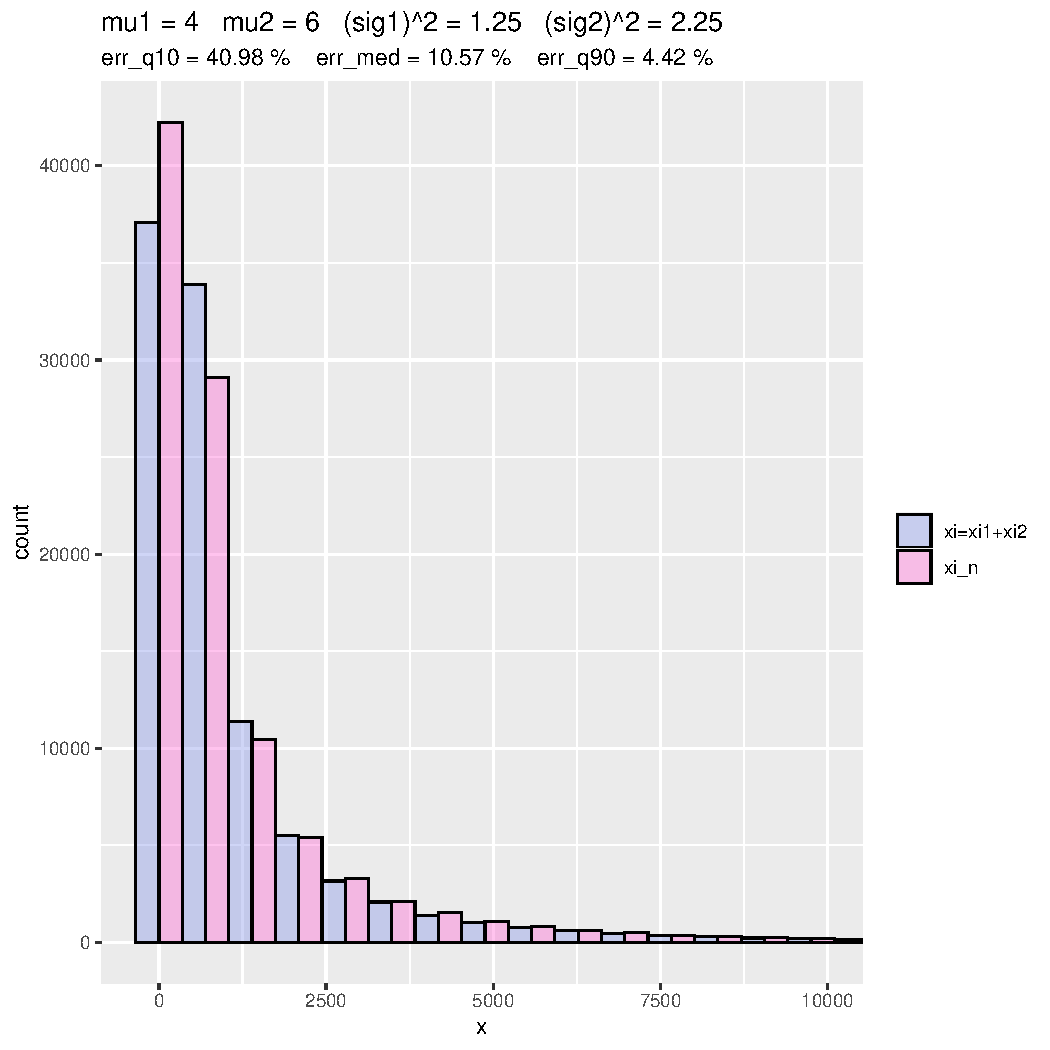
\includegraphics[width=1\linewidth]{hist_new_2.pdf}
				\caption{Сумма логнормальных.} %% подпись к рисунку
				\label{ris7} %% метка рисунка для ссылки на него
			\end{minipage}
			
		\end{center}
	\end{figure}	
	
\end{frame}

\begin{frame}{Точность аппроксимации }
	
	\begin{figure}[h]
		\begin{center}
			\begin{minipage}[h]{0.8\linewidth}
				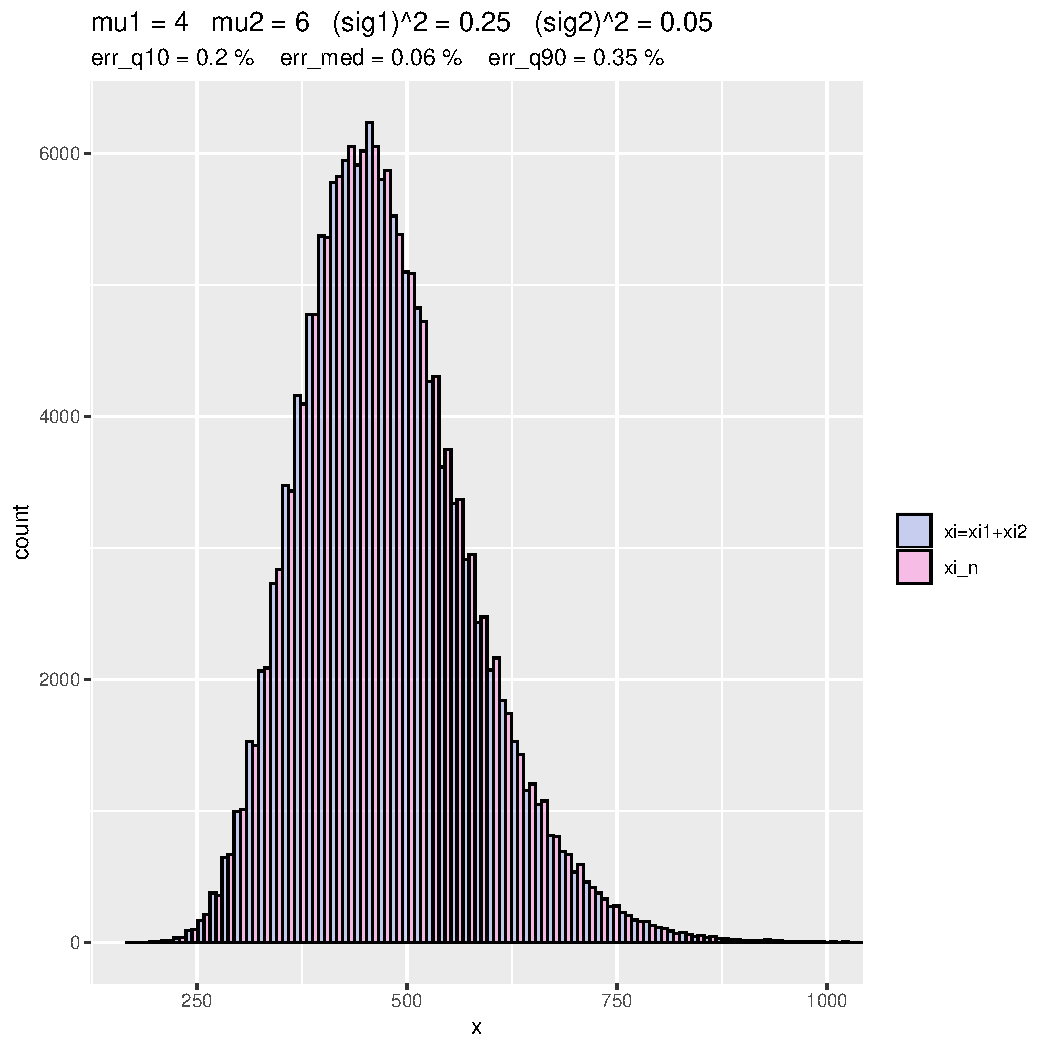
\includegraphics[width=1\linewidth]{hist_new_3.pdf}
				\caption{Сумма логнормальных.} %% подпись к рисунку
				\label{ris7} %% метка рисунка для ссылки на него
			\end{minipage}
			
		\end{center}
	\end{figure}	
	
\end{frame}

\begin{frame}{Точность аппроксимации }
	
	\begin{figure}[h]
		\begin{center}
			\begin{minipage}[h]{0.8\linewidth}
				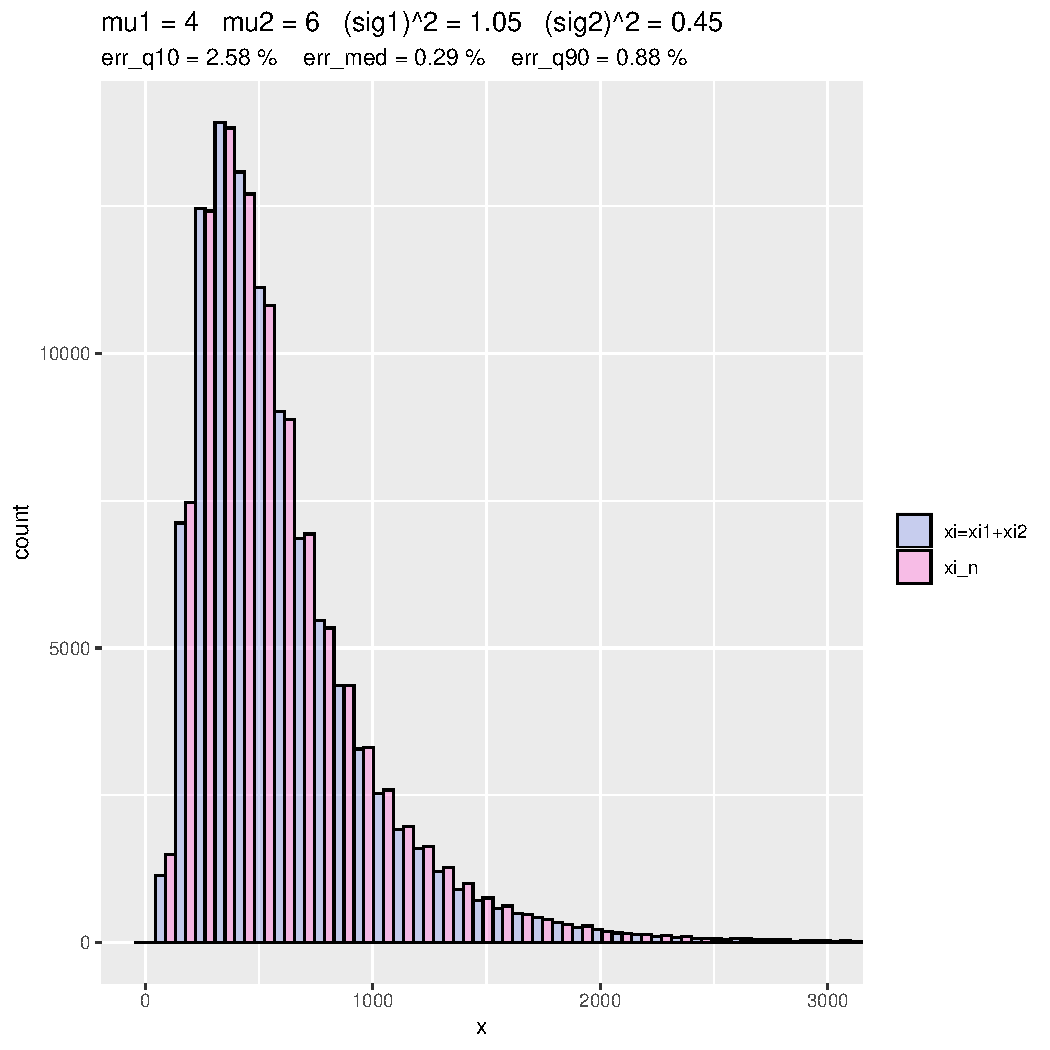
\includegraphics[width=1\linewidth]{hist_new_4.pdf}
				\caption{Сумма логнормальных.} %% подпись к рисунку
				\label{ris7} %% метка рисунка для ссылки на него
			\end{minipage}
			
		\end{center}
	\end{figure}	
	
\end{frame}

\begin{frame}{}
	
	
	\textcolor{blue}{\hbox{\textbf{Результаты:}}}
	\begin{enumerate}
		\item Методы аппроксимации нормального, логнормального распределений.
		\item Условие на $\sigma$ для аппроксимации.
		\item Точность аппроксимации логнормального правилом 30-40-30.
		\item Метод аппроксимации произведения логнормальных распределений.
		\item Метод аппроксимации суммы логнормальных распределений.
		\item Точность аппроксимации суммы логнормальных распределений.
	\end{enumerate}
	\bigskip
	\textcolor{blue}{\hbox{\textbf{Проблемы:}}}
	\begin{enumerate}
		\item Аппроксимировать дискретным распределением получается только при ограниченных $\sigma$.
		\item  Для суммы логнормальных результат имеет ошибки, так как сумма логнормальных не логнормальная.
	\end{enumerate}
	
\end{frame}


	
	
\end{document}